

% make text 4.16'' x 7''
% fleqn, leqno

\documentclass[twoside,11pt]{article}

\usepackage[utf8]{inputenc}

\usepackage[%
%paperwidth=5.16in,
paperwidth=5.5in,
paperheight=8.5in,
left=.5in,
right=.5in,
bottom=.5in,
top=1in % typically =1in, but changing temporarily...
]{geometry}
%

%\renewcommand{\numberline}[1]{#1~}



% we want to indent first paragraphs
\usepackage{indentfirst}

% typography tools
\linespread{.9}
\usepackage{microtype}

% set paragraph indentation
\setlength{\parindent}{2em}


% for section numbering
\usepackage[]{titlesec} 
\newcommand{\periodafter}[1]{#1.}

%\titleformat{\chapter}%
%{\centering\normalsize\sc}
%{\thechapter\periodafter}{1em}{}

\titleformat{\section}%
{\centering\normalsize\sc}
{\thesection\periodafter}{1em}{}

\titleformat{\subsection}%
{\normalsize\itshape}
{\thesection.\thesubsection\periodafter}{1em}{}

\titleformat{\subsubsection}%
{\normalsize\itshape}
{\thesection.\thesubsection.\thesubsubsection\periodafter}{1em}{}


%\renewcommand{\thechapter}{\Roman{chapter}}
\renewcommand{\thesection}{\Roman{section}}
\renewcommand{\thesubsection}{\Alph{subsection}}
\renewcommand{\thesubsubsection}{\roman{subsubsection}}






%----------------------------------
% NEW CENTURY SCHOOLBOOK (QJE)
\usepackage{fouriernc}
\usepackage[cal=cm]{mathalpha} % I prefer these mathcal letters




%=====================================================================
% Stuff for getting the content how you want it


%\usepackage[T1]{fontenc} % hyphenation for accented characters?
\usepackage{mathtools}
\usepackage{enumitem} %\begin{enumerate}[label=Case \arabic*., align=left, leftmargin=*]
\usepackage{amsthm}
   \newtheorem{theorem}{Theorem}
   \newtheorem{prop}{Proposition}
   \newtheorem{lemma}{Lemma}
   \newtheorem{coro}{Corollary}
\usepackage{commath} % calculus: \dif (also has mixed partial derivative...)
\usepackage{tcolorbox} % inset boxes
\usepackage{physics} % for \dv and \pdv
   \newcommand{\wpdv}[2]{\partial #1 / \partial #2}
\usepackage{natbib}
   \bibliographystyle{authordate1}

\usepackage{centernot} % for \centernot\implies
\newcommand{\nimplies}{\centernot\implies}

\usepackage{float}
\usepackage{graphicx}
\usepackage{subcaption}
%\usepackage{subfig} % could be useful for some journals

\usepackage{booktabs}
\usepackage{tabularx}
\newcolumntype{Y}{>{\raggedleft\arraybackslash}X}
\newcolumntype{C}{>{\centering\arraybackslash}X}
\newcommand{\ra}[1]{\renewcommand{\arraystretch}{#1}}

% Redefining the abstract to have width=\textwidth
\renewenvironment{abstract}
  {\noindent
   \begin{minipage}[t]{\textwidth}
   \setlength{\parindent}{2em}
   \renewcommand{\baselinestretch}{1.0}
   \footnotesize}
  {\end{minipage}}
  
  
%=====================================================================
% Some stuff for captioning figures
\usepackage[%
format=plain,
labelformat=simple,
labelsep=newline,
justification=centerfirst,
labelfont={footnotesize,sc},
textfont={footnotesize}
]{caption}
\setlength{\abovecaptionskip}{8pt plus 0pt minus 2pt}
%\setlength{\abovecaptionskip}{0pt}
\setlength{\belowcaptionskip}{-2pt}

\newcommand{\mycaption}[2]{%
	\caption[#1]{%
		\begin{minipage}[]{\textwidth}
		\setlength{\parindent}{1em}
		\vspace{.25cm}
		\begin{center}
		#1
		\end{center}
		\vspace{-.25cm}
		
		#2
		\end{minipage}
	}
}

\renewcommand{\thetable}{\Roman{table}}
\renewcommand{\thefigure}{\Roman{figure}}
\renewcommand{\thesubtable}{\Alph{subtable}}
\renewcommand{\thesubfigure}{\Alph{subfigure}}

\usepackage[dotinlabels]{titletoc}

\dottedcontents{section}% section
               [3em]% how far in (from margin) do you want the title to start?
               {\addvspace{.5em}\footnotesize\sc}% before-code
               {3em}% how far back (from the title words) do you want the number to appear?
               {0.75em}% how much elbow-room do the dots require

\dottedcontents{subsection}%
               [6em]%
               {\addvspace{.25em}\footnotesize\itshape}%
               {3em}%
               {0.75em}

\dottedcontents{subsubsection}%
               [9em]%
               {\addvspace{.25em}\footnotesize\itshape}%
               {3em}%
               {0.75em}

\setcounter{tocdepth}{3}

%=====================================================================
% Useful macros

\renewcommand{\L}{\mathcal{L}}
\newcommand{\U}{\mathcal{U}}

\newcommand{\R}{\mathbb{R}}
\newcommand{\N}{\mathbb{N}}
\newcommand{\Z}{\mathbb{Z}}

\newcommand{\E}{E}
\newcommand{\giv}{\;|\;}
\newcommand{\eps}{\varepsilon}

%\usepackage{amsmath}
\DeclareMathOperator*{\argmax}{arg\,max}
\DeclareMathOperator*{\argmin}{arg\,min}
\DeclareMathOperator{\sign}{sgn}

\renewcommand{\dot}[1]{\overset{\textrm{\large{.}}}{#1}}

%=====================================================================
% Latin macros

\newcommand{\ie}{\emph{i.e.},~}
\newcommand{\Ie}{\emph{I.e.},~}
\newcommand{\eg}{\emph{e.g.}~}
\newcommand{\cetpar}{\emph{cet. par.},~}
\newcommand{\parpas}{\emph{pari passu}~}
\newcommand{\qua}{\emph{quaesitum}~}

%=====================================================================
% Shortcuts for brackets/parentheses of different sizes

\newcommand{\bigb}[1]{\big[ #1 \big]}
\newcommand{\Bigb}[1]{\Big[ #1 \Big]}
\newcommand{\biggb}[1]{\bigg[ #1 \bigg]}
\newcommand{\Biggb}[1]{\Bigg[ #1 \Bigg]}

\newcommand{\bigp}[1]{\big( #1 \big)}
\newcommand{\Bigp}[1]{\Big( #1 \Big)}
\newcommand{\biggp}[1]{\bigg( #1 \bigg)}
\newcommand{\Biggp}[1]{\Bigg( #1 \Bigg)}

\newcommand{\bigc}[1]{\big\{ #1 \big\}}
\newcommand{\Bigc}[1]{\Big\{ #1 \Big\}}
\newcommand{\biggc}[1]{\bigg\{ #1 \bigg\}}
\newcommand{\Biggc}[1]{\Bigg\{ #1 \Bigg\}}


%=====================================================================
% Not sure how this works, but it pushes stuff to the right if you need that within align.

\makeatletter
\newcommand{\pushright}[1]{\ifmeasuring@#1\else\omit\hfill$\displaystyle#1$\fi\ignorespaces}
\newcommand{\pushleft}[1]{\ifmeasuring@#1\else\omit$\displaystyle#1$\hfill\fi\ignorespaces}
\makeatother



\usepackage{xcolor}

% lighter color palette
\definecolor{OperaBlue}{HTML}{87A7B7}
\definecolor{OperaMauve}{HTML}{B784A7}
\definecolor{OperaGreen}{HTML}{A7B784}

% preferred triadic color palette
\definecolor{BlueTaupe}{HTML}{5F6D91}
\definecolor{MauveTaupe}{HTML}{915F6D}
\definecolor{GreenTaupe}{HTML}{6D915F}

% darker color palette
\definecolor{OldBlue}{HTML}{314767}
\definecolor{OldMauve}{HTML}{673147}
\definecolor{OldGreen}{HTML}{476731}


% Cambridge color scheme
\definecolor{CamRed}{HTML}{D50032}
\definecolor{CamBlue}{HTML}{0072CE}
\definecolor{CamOrange}{HTML}{E87722}
\definecolor{CamGreen}{HTML}{64A70B}
\definecolor{CamPurple}{HTML}{93328E}
\definecolor{CamTeal}{HTML}{00B0B9}


\usepackage{hyperref}
\hypersetup{
  colorlinks = true, %Colours links instead of ugly boxes
  urlcolor   = blue, %Colour for external hyperlinks
  linkcolor  = blue, %Colour of internal links
  citecolor  = blue  %Colour of citations
}
\usepackage[nameinlink,noabbrev]{cleveref}






\usepackage{tikz}

%\usepackage{pgfplots}
%\usepgfplotslibrary{fillbetween}
%\pgfplotsset{compat = newest}

\newpagestyle{main}{
  \sethead
    [\thepage][\textit{\footnotesize{DIAGRAM}}][]  % even
    {}{\textit{\footnotesize{DIAGRAM}}}{\thepage}} % odd
\pagestyle{main}

\usetikzlibrary{decorations.pathreplacing,angles,quotes}


\begin{document}

When we use \texttt{ADOL-C} to differentiate a function with respect to $n$ variables, with maximum degree $d$, we can consider the combinatorics problem of choosing $d$ elements from a set of $n+1$ elements, where repetitions are allowed.
Note that the ``extra'' element corresponds to the null variable, for which we do not differentiate.
Therefore, upon performing the differentiation, we expect the number of values to be given by:
\[
N = \biggp{\begin{array}{c} (n+1)+d-1 \\ d \end{array}} = 
    \biggp{\begin{array}{c} n+d \\ d \end{array}} = 
    \frac{(n+d)!}{(d)!(n)!}.
\]

On one hand, the data is 5D, but \texttt{ADOL-C} thinks it's 3D, and uses a 2D storage method.
On the other hand, we would like to make use of the dimensions that \texttt{ADOL-C} doesn't know about, and we would then like to permute the tensor, and use our own 2D storage method.
To top matters off, the 2D storage used by \texttt{ADOL-C} is more efficient than we need, so the mapping is not a function (since most of their values map to more than one of our storage locations). 

\[
\left[
\begin{array}{ccc|ccc|c|ccc}
\pdv{F_{1}}{r_{1}}{c_{1}} & \cdots & \pdv{F_{1}}{r_{1}}{c_{q}} &
\pdv{F_{1}}{r_{2}}{c_{1}} & \cdots & \pdv{F_{1}}{r_{2}}{c_{q}} & \cdots & 
\pdv{F_{1}}{r_{p}}{c_{1}} & \cdots & \pdv{F_{1}}{r_{p}}{c_{q}} \\
%
\pdv{F_{2}}{r_{1}}{c_{1}} & \cdots & \pdv{F_{2}}{r_{1}}{c_{q}} &
\pdv{F_{2}}{r_{2}}{c_{1}} & \cdots & \pdv{F_{2}}{r_{2}}{c_{q}} & \cdots & 
\pdv{F_{2}}{r_{p}}{c_{1}} & \cdots & \pdv{F_{2}}{r_{p}}{c_{q}} \\
%
\vdots & & \vdots & \vdots & & \vdots & & \vdots & & \vdots \\
%
\pdv{F_{n}}{r_{1}}{c_{1}} & \cdots & \pdv{F_{n}}{r_{1}}{c_{q}} &
\pdv{F_{n}}{r_{2}}{c_{1}} & \cdots & \pdv{F_{n}}{r_{2}}{c_{q}} & \cdots & 
\pdv{F_{n}}{r_{p}}{c_{1}} & \cdots & \pdv{F_{n}}{r_{p}}{c_{q}}
\end{array}
\right]
\]


%This interpretation suggests organizing the values into a multi-dimensional array, where each degree of differentiation corresponds to a dimension of the array, and traversing a given dimension enumerates the different variables.

%We consider an example where the maximum degree of differentiation is 2, and there are 6 variables with respect to which we can differentiate. Using the above formula, we recognize that there will be 28 ways to differentiate our function. Recognize that as long as the vector containing the indices is ``non-increasing,'' (e.g. element 12 is given by $(4,2)$, where $4 > 2$) that we do not need to know the total number of variables.

%In practice, we will give the function $d$ as well, however this should only be used in order to know the length of the array of indices.

%One of our initial challenges in solving the model is to construct arrays of 



\begin{figure}
\centering

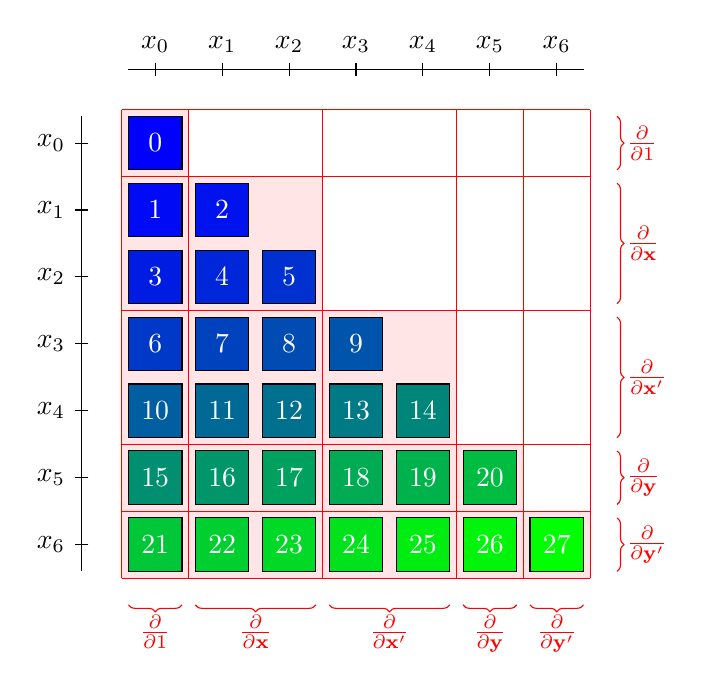
\begin{tikzpicture}[scale=0.85]

\filldraw[color=red!10, fill=red!10] (-.1,-.1) rectangle (6.9,0.9);
\filldraw[color=red!10, fill=red!10] (-.1,0.9) rectangle (5.9,1.9);
\filldraw[color=red!10, fill=red!10] (-.1,1.9) rectangle (4.9,3.9);
\filldraw[color=red!10, fill=red!10] (-.1,3.9) rectangle (2.9,5.9);
\filldraw[color=red!10, fill=red!10] (-.1,5.9) rectangle (0.9,6.9);

\draw[red, solid] (-.1,-.1) -- (6.9,-.1);
\draw[red, solid] (-.1,0.9) -- (6.9,0.9);
\draw[red, solid] (-.1,1.9) -- (6.9,1.9);
\draw[red, solid] (-.1,3.9) -- (6.9,3.9);
\draw[red, solid] (-.1,5.9) -- (6.9,5.9);
\draw[red, solid] (-.1,6.9) -- (6.9,6.9);

\draw[red, solid] (-.1,-.1) -- (-.1,6.9);
\draw[red, solid] (0.9,-.1) -- (0.9,6.9);
\draw[red, solid] (2.9,-.1) -- (2.9,6.9);
\draw[red, solid] (4.9,-.1) -- (4.9,6.9);
\draw[red, solid] (5.9,-.1) -- (5.9,6.9);
\draw[red, solid] (6.9,-.1) -- (6.9,6.9);


\filldraw[color=black, fill=green!0!blue] (0,6) rectangle node[text=white]{0} (.8,6.8);

\filldraw[color=black, fill=green!4!blue] (0,5) rectangle node[text=white]{1} (.8,5.8);
\filldraw[color=black, fill=green!7!blue] (1,5) rectangle node[text=white]{2} (1.8,5.8);

\filldraw[color=black, fill=green!11!blue] (0,4) rectangle node[text=white]{3} (.8,4.8);
\filldraw[color=black, fill=green!15!blue] (1,4) rectangle node[text=white]{4} (1.8,4.8);
\filldraw[color=black, fill=green!19!blue] (2,4) rectangle node[text=white]{5} (2.8,4.8);

\filldraw[color=black, fill=green!22!blue] (0,3) rectangle node[text=white]{6} (.8,3.8);
\filldraw[color=black, fill=green!26!blue] (1,3) rectangle node[text=white]{7} (1.8,3.8);
\filldraw[color=black, fill=green!30!blue] (2,3) rectangle node[text=white]{8} (2.8,3.8);
\filldraw[color=black, fill=green!33!blue] (3,3) rectangle node[text=white]{9} (3.8,3.8);

\filldraw[color=black, fill=green!37!blue] (0,2) rectangle node[text=white]{10} (.8,2.8);
\filldraw[color=black, fill=green!41!blue] (1,2) rectangle node[text=white]{11} (1.8,2.8);
\filldraw[color=black, fill=green!44!blue] (2,2) rectangle node[text=white]{12} (2.8,2.8);
\filldraw[color=black, fill=green!48!blue] (3,2) rectangle node[text=white]{13} (3.8,2.8);
\filldraw[color=black, fill=green!52!blue] (4,2) rectangle node[text=white]{14} (4.8,2.8);

\filldraw[color=black, fill=green!56!blue] (0,1) rectangle node[text=white]{15} (.8,1.8);
\filldraw[color=black, fill=green!59!blue] (1,1) rectangle node[text=white]{16} (1.8,1.8);
\filldraw[color=black, fill=green!63!blue] (2,1) rectangle node[text=white]{17} (2.8,1.8);
\filldraw[color=black, fill=green!67!blue] (3,1) rectangle node[text=white]{18} (3.8,1.8);
\filldraw[color=black, fill=green!70!blue] (4,1) rectangle node[text=white]{19} (4.8,1.8);
\filldraw[color=black, fill=green!74!blue] (5,1) rectangle node[text=white]{20} (5.8,1.8);

\filldraw[color=black, fill=green!78!blue] (0,0) rectangle node[text=white]{21} (.8,.8);
\filldraw[color=black, fill=green!81!blue] (1,0) rectangle node[text=white]{22} (1.8,.8);
\filldraw[color=black, fill=green!85!blue] (2,0) rectangle node[text=white]{23} (2.8,.8);
\filldraw[color=black, fill=green!89!blue] (3,0) rectangle node[text=white]{24} (3.8,.8);
\filldraw[color=black, fill=green!93!blue] (4,0) rectangle node[text=white]{25} (4.8,.8);
\filldraw[color=black, fill=green!96!blue] (5,0) rectangle node[text=white]{26} (5.8,.8);
\filldraw[color=black, fill=green!100!blue] (6,0) rectangle node[text=white]{27} (6.8,.8);

\draw (0,7.5) -- (6.8,7.5);
\draw (0.4,7.4) -- (0.4,7.6) node[anchor=south]{$x_{0}$};
\draw (1.4,7.4) -- (1.4,7.6) node[anchor=south]{$x_{1}$};
\draw (2.4,7.4) -- (2.4,7.6) node[anchor=south]{$x_{2}$};
\draw (3.4,7.4) -- (3.4,7.6) node[anchor=south]{$x_{3}$};
\draw (4.4,7.4) -- (4.4,7.6) node[anchor=south]{$x_{4}$};
\draw (5.4,7.4) -- (5.4,7.6) node[anchor=south]{$x_{5}$};
\draw (6.4,7.4) -- (6.4,7.6) node[anchor=south]{$x_{6}$};

\draw (-.7,0) -- (-.7,6.8);
\draw (-.6,6.4) -- (-.8,6.4) node[anchor=east]{$x_{0}$};
\draw (-.6,5.4) -- (-.8,5.4) node[anchor=east]{$x_{1}$};
\draw (-.6,4.4) -- (-.8,4.4) node[anchor=east]{$x_{2}$};
\draw (-.6,3.4) -- (-.8,3.4) node[anchor=east]{$x_{3}$};
\draw (-.6,2.4) -- (-.8,2.4) node[anchor=east]{$x_{4}$};
\draw (-.6,1.4) -- (-.8,1.4) node[anchor=east]{$x_{5}$};
\draw (-.6,0.4) -- (-.8,0.4) node[anchor=east]{$x_{6}$};

\draw[decoration={brace,mirror},decorate,color=red] (0, -.5) -- node[anchor=north] {$\frac{\partial}{\partial 1}$} (0.8,-.5);
\draw[decoration={brace,mirror},decorate,color=red] (1, -.5) -- node[anchor=north] {$\frac{\partial}{\partial \mathbf{x}}$} (2.8,-.5);
\draw[decoration={brace,mirror},decorate,color=red] (3, -.5) -- node[anchor=north] {$\frac{\partial}{\partial \mathbf{x}'}$} (4.8,-.5);
\draw[decoration={brace,mirror},decorate,color=red] (5, -.5) -- node[anchor=north] {$\frac{\partial}{\partial \mathbf{y}}$} (5.8,-.5);
\draw[decoration={brace,mirror},decorate,color=red] (6, -.5) -- node[anchor=north] {$\frac{\partial}{\partial \mathbf{y}'}$} (6.8,-.5);

\draw[decoration={brace,mirror},decorate,color=red] (7.3, 0) -- node[anchor=west] {$\frac{\partial}{\partial \mathbf{y}'}$} (7.3,0.8);
\draw[decoration={brace,mirror},decorate,color=red] (7.3, 1) -- node[anchor=west] {$\frac{\partial}{\partial \mathbf{y}}$} (7.3,1.8);
\draw[decoration={brace,mirror},decorate,color=red] (7.3, 2) -- node[anchor=west] {$\frac{\partial}{\partial \mathbf{x}'}$} (7.3,3.8);
\draw[decoration={brace,mirror},decorate,color=red] (7.3, 4) -- node[anchor=west] {$\frac{\partial}{\partial \mathbf{x}}$} (7.3,5.8);
\draw[decoration={brace,mirror},decorate,color=red] (7.3, 6) -- node[anchor=west] {$\frac{\partial}{\partial 1}$} (7.3,6.8);

\end{tikzpicture}

\mycaption{\texttt{ADOL-C} Arrangement}{If $n_{x} = 2$ and $n_{y} = 1$, then there are 6 variables with respect to which we can differentiate 0, 1, or 2 times.}
\label{fig1}
\end{figure}

\end{document}
